\documentclass{cis320}
\usepackage{listings}
\usepackage{xcolor}
\usepackage{lmodern}
\usepackage{listings}
\usepackage{physics}
\usepackage{graphicx}
\usepackage{subfig}

%New colors defined below
\definecolor{codegreen}{rgb}{0,0.6,0}
\definecolor{codegray}{rgb}{0.5,0.5,0.5}
\definecolor{codepurple}{rgb}{0.58,0,0.82}
\definecolor{backcolour}{rgb}{0.95,0.95,0.92}

%Code listing style named "mystyle"
\lstdefinestyle{mystyle}{
  backgroundcolor=\color{backcolour}, commentstyle=\color{codegreen},
  keywordstyle=\color{magenta},
  numberstyle=\tiny\color{codegray},
  stringstyle=\color{codepurple},
  basicstyle=\ttfamily\footnotesize,
  breakatwhitespace=false,         
  breaklines=true,                 
  numbers=none,             
  keepspaces=true,                                     
  numbersep=5pt,                  
  showspaces=false,
  language=[90]Fortran,                
  showstringspaces=false,
  showtabs=false,                  
  tabsize=2
}
\lstset{style=mystyle}
\addbibresource{./Sources.bib}

\begin{document}
\noindent Homework \textbf{LTTC Quantum dynamics}\hfill  Mauro Gascon Navas\\
TCCM \today

\hrulefill
\par
\vspace{1cm} 
All fll scripts and files generated while completing each homework can be found in its this \textcolor{blue}{\href{https://github.com/EliteSushi/LTTC2025/tree/main/Quantum_Dynamics}{Github repository}}.

\section{Hermite Polynomials Function}

To calculculate the hermite polynomials, a recursive function can be used. The function calls itself to calculate $H_{n-1}(y)$ and $H_{n-2}(y)$ until reaching $H_1(y)=1$ and $H_0(y)=2y$, where its values are set and the recursion loop is exited. In the code propagate, the functions are written in a module called \textit{functions2use}.\\
Something worth noting, is that at each step of the recursion, the function is called twice, so the complexity of the function is $O(2^n)$, which is not ideal for large $n$. This contrasts to e.g. a factorial function (which is also typically written as a recursive function), where its complexity goes as $O(n)$.\\
\par 
The function taks two inputs: the order of the polynomial (n) and the point to evaluate (y), and outputs one result (h).
    \begin{lstlisting}[caption=Recursive function to calculate hermite polynomials]
recursive function hermite(n,y) result(h) 
!Recursive function to calculate the hermite polynomials
    implicit none

    integer, intent(in) :: n
    real(8), intent(in) :: y
    real(8) :: h

    if (n<0) then !Check for proper usage
    write(*,*) "Error in hermite: n must be <=0"
    h=0.d0
    endif

    if (n==0) then !If statements to end recursion
    h=1.d0
    elseif (n==1) then
    h=2.d0*y
    else
    h=2.d0*y*hermite(n-1,y)-2.d0*(n-1)*hermite(n-2,y) !Recursion
    endif
end function hermite \end{lstlisting}

\section*{2 3 4 \quad Wavefunction initialization}
\setcounter{section}{4}
The \textit{initpsi} subroutine is modified so that the wavefunction is initialized as a weighted sum of the harmonic eigenfunctions. To make it as general as possible, first the number of eigenfunctions to use (\textit{ncoeff}) is read from the input file \textit{wavefunction}. Then the coefficients for each parent eigenfunction are read and stored as an array (\textit{coeff}) in a sequential manner. In \textit{initpsi}, \textit{coeff} is looped over.\\
Finally, the wavefunction is normalized exploiting the fact that the eigenfunctions are orthogonal to eachother: $N^2 = \Sigma_i c_i^2$.\\
\par
The modified subroutine takes as inputs: \textit{npoints} (x axis grid), \textit{dx} (grid spacing), \textit{x0} (center of the wavefunction), \textit{psi0} (wavefunction array), \textit{ncoeff} (number of eigenfunctions), \textit{coeff} (ordered array with the eigenfuction coefficients).

    \begin{lstlisting}[caption=Modified \textit{initpsi} subroutine]
subroutine initpsi(npoints,dx,x0,psi0,ncoeff,coeff)      
!Modified initpsi to initiate wavefunction expanded in the harmonic eigenfunctions
    use parameters
    use functions2use
    implicit none
    
    integer :: i,j,l,npoints,ncoeff
    real(8) :: x,x0,dx,mo,sqmopi,sqmo,A,coeff(ncoeff), N
    complex(8) :: psi0(npoints), res
    
    mo = mass*angfreq !Constants that will be needed in the loop
    sqmo = sqrt(mo) 
    sqmopi = sqmo/sqrt(pi)
    psi0 = (0.d0,0.d0) 
    do l = 0, ncoeff-1 !Loop through the user specified eigenfunctions
        if (coeff(l+1)==0) cycle !if Coefficient = 0 skip
        A = sqrt(1.d0/(2.d0**l*dble(gamma(real(l+1))))*sqmopi) !Constant
        do i=-npoints/2+1,npoints/2
            x=dble(i)*dx
            if (i>0) then
            j=i
            else     
            j=i+npoints
            endif
            res = coeff(l+1)*A*exp(-mo*(x-x0)**2/2.d0)*hermite(l,(x-x0)*sqmo) !coefficient*Eigenfucntion
            psi0(j) = psi0(j) + res
        end do
    enddo
    
    N = sqrt(sum(coeff**2))!Normalize eigenfunction
    psi0 = psi0 / N 
end subroutine initpsi\end{lstlisting}

The initial coefficients are read from the \textit{wavefunction} file by modifying the main propgram \textit{propagate}: The added arguments are the number of eigenfunctions to use (\textit{ncoeff}), which is also the highest eigenfunction order, followed by the cefficients, one at each line.
Additionally, to make the outputs lighter, a snapshot frequency is also added, it will only output the positions every \textit{snapshot} steps. 
    \begin{lstlisting}[caption=Reading the coefficients in the main program]
open(unit=10,file='wavepacket') ! User specified eigenfunctions/coefficents
    ...
    read(10,*) snapshot              !snapshot frequency
    read(10,*) ncoeff                !Number of coefficients
    allocate(coeff(ncoeff))          !Initialize coeff array
    coeff=0.d0
    do i = 1, ncoeff                 !Read ncoeff coefficients or until EOF 
        read(10,*,iostat=iostat) coeff(i)
        if (iostat /= 0) exit 
    end do
close(10) \end{lstlisting}

    \begin{lstlisting}[language=bash, caption=Wavefunction input file]
512     #Number of lattice points
-0.0    #Initial position (in Bohr)
12.755  #Governs the initial width of the wave packet (in Bohr^(-2))
0.01    #Propagation time step (in fs)
4000    #Number of propagation steps
20      #Snapshot frequency (after 20 timesteps a snapshot will be taken)
3       #Number of Coefficients
1       #c0
1       #c1
0       #c2\end{lstlisting}

Finally, though not shown, for convenience the plotting subroutines were rewritten to use gnuplot.

\section{Pure Eigenfunctions}
For pure eigenfunctions, the probability density of the pure eigenfunctions remains static:
\[
\Psi_{n}(x,t) = e^{-iE_nt} \cdot \Phi_{n}(x) = e^{-it\omega(n+\frac{1}{2})} \cdot \Phi_{n}(x) 
\]\[
 \abs{\Psi_{n}(x,t)}^2 = [ e^{itE_n} \cdot \Phi_{n}(x)][e^{-itE_n} \cdot \Phi_{n}(x)] = \abs{\Phi_n(x)}^2 
\]

\begin{figure}[h]
    \centering
    \subfloat[$\Phi_0$]{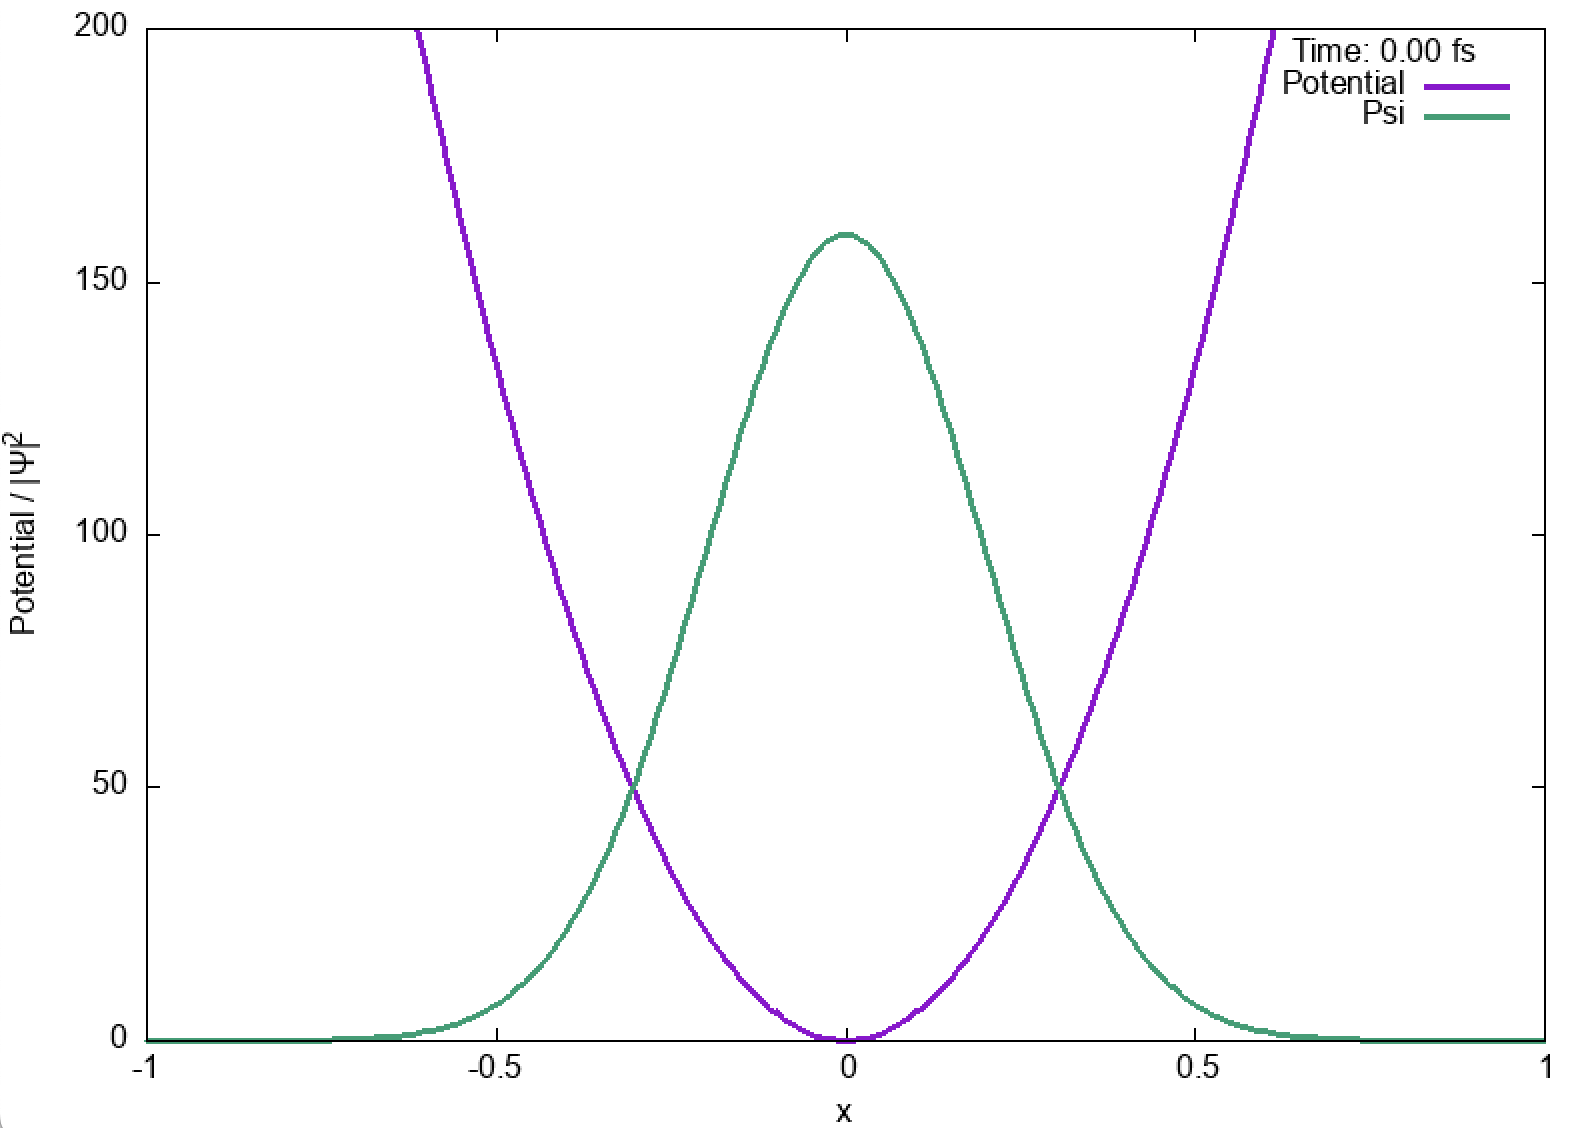
\includegraphics[width=0.33\textwidth]{H0.png}}
    \subfloat[$\Phi_1$]{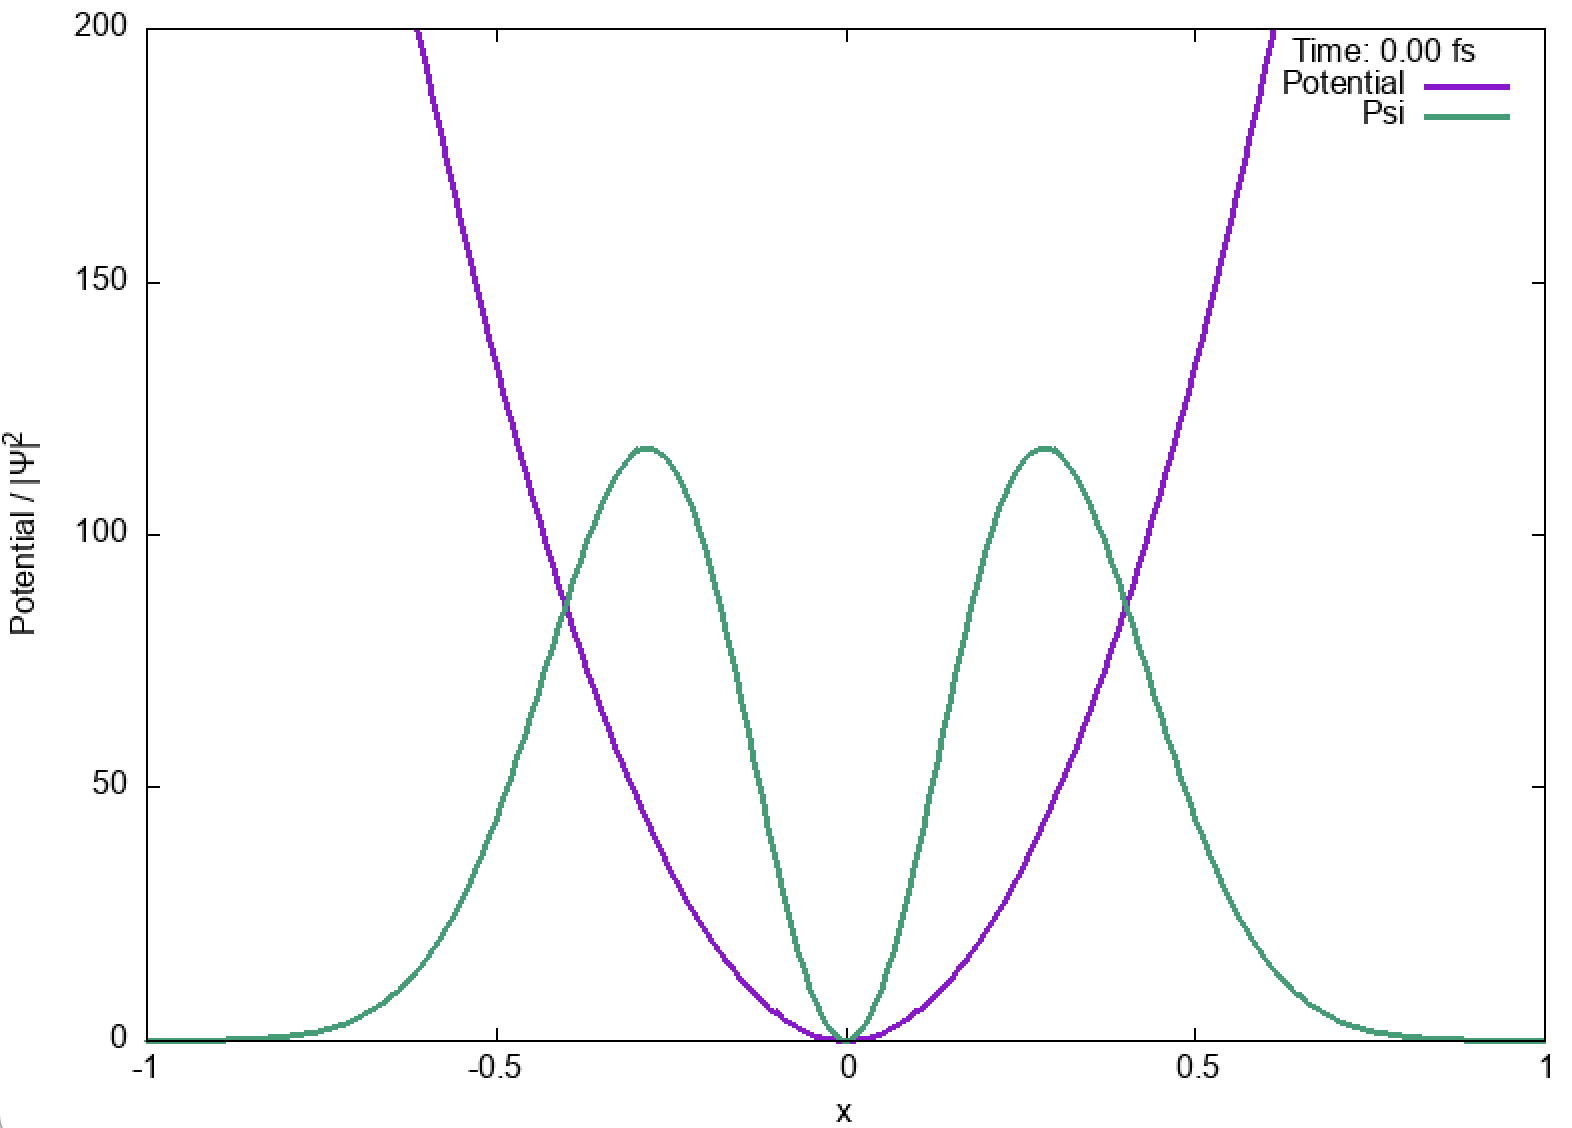
\includegraphics[width=0.33\textwidth]{H1.png}}
    \subfloat[$\Phi_2$]{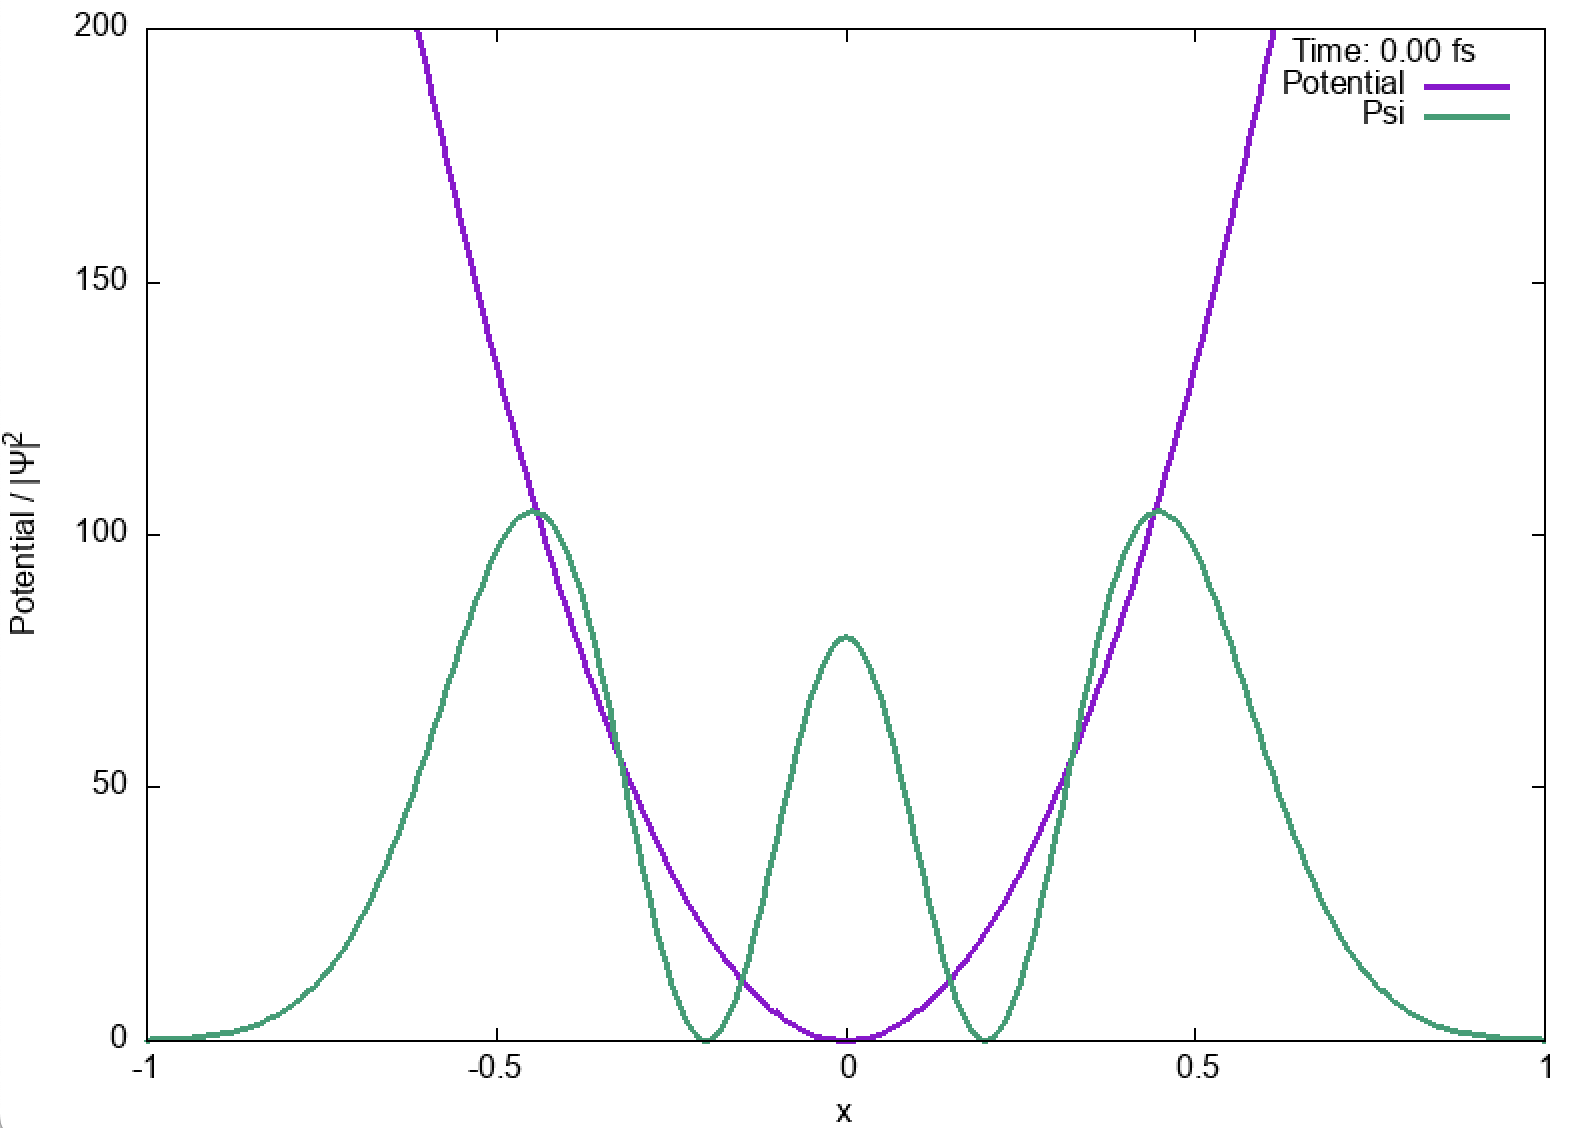
\includegraphics[width=0.33\textwidth]{H2.png}}
    \vspace{0.5cm}
    \subfloat[$\Phi_3$]{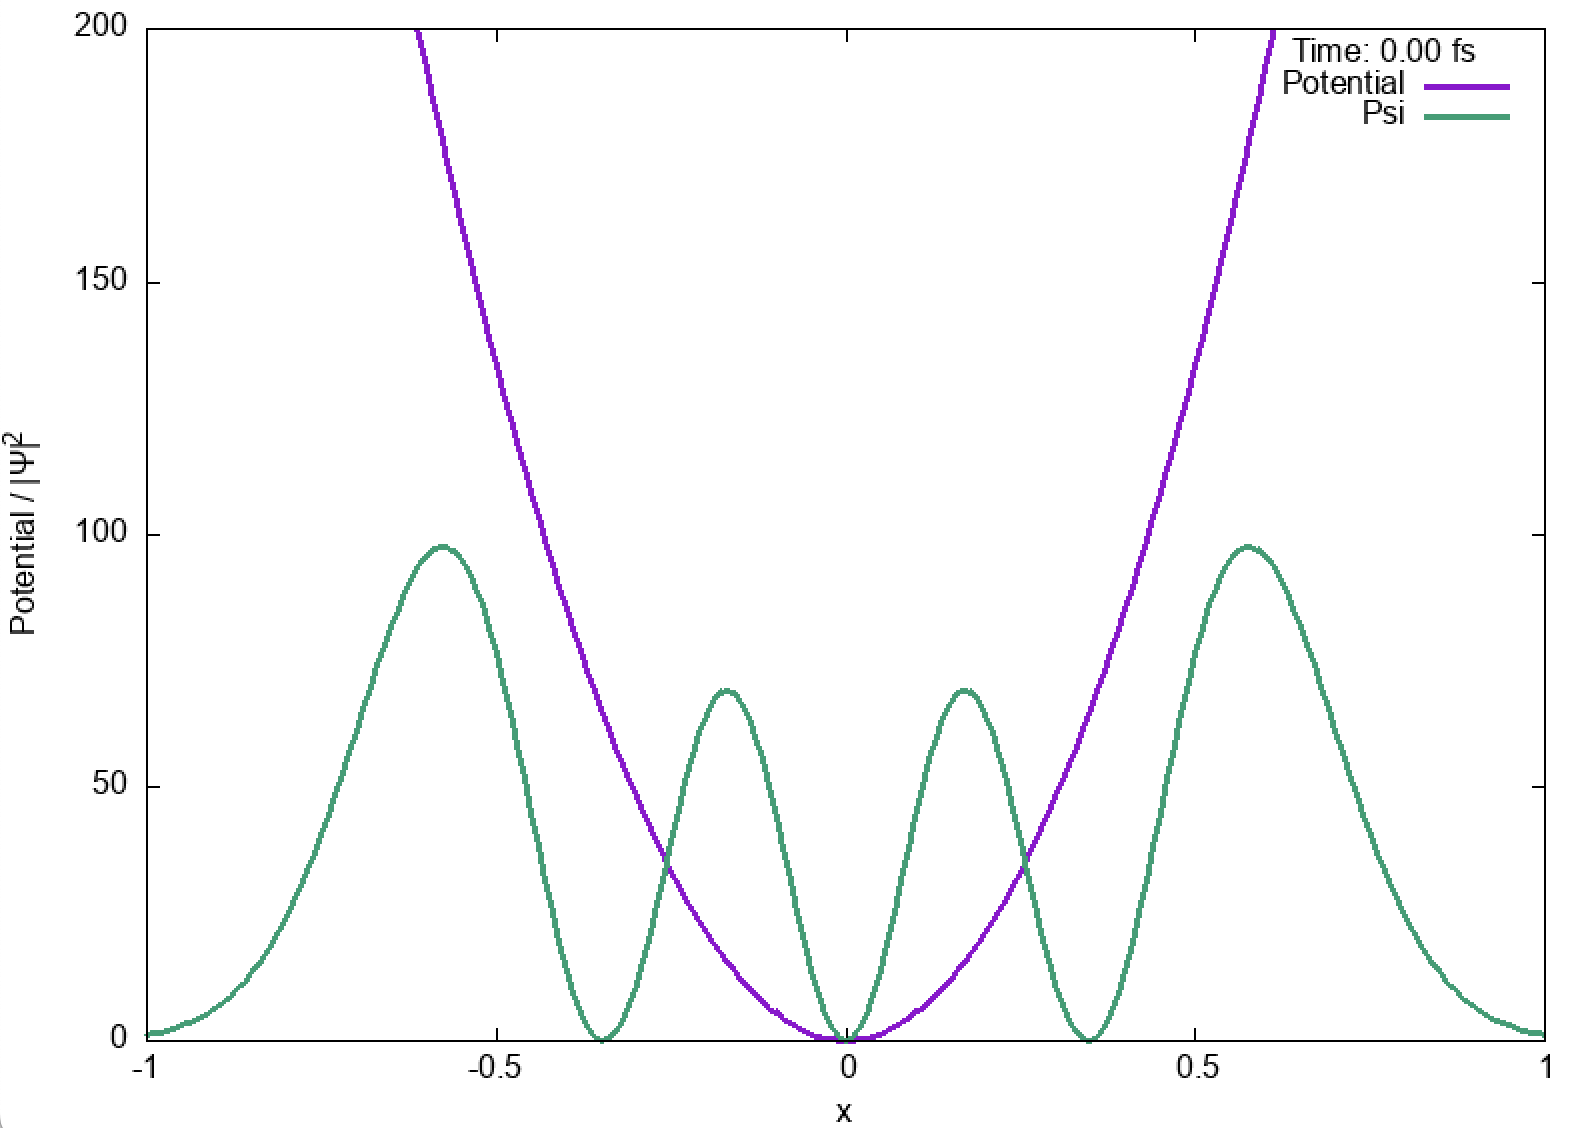
\includegraphics[width=0.33\textwidth]{H3.png}}
    \subfloat[$\Phi_4$]{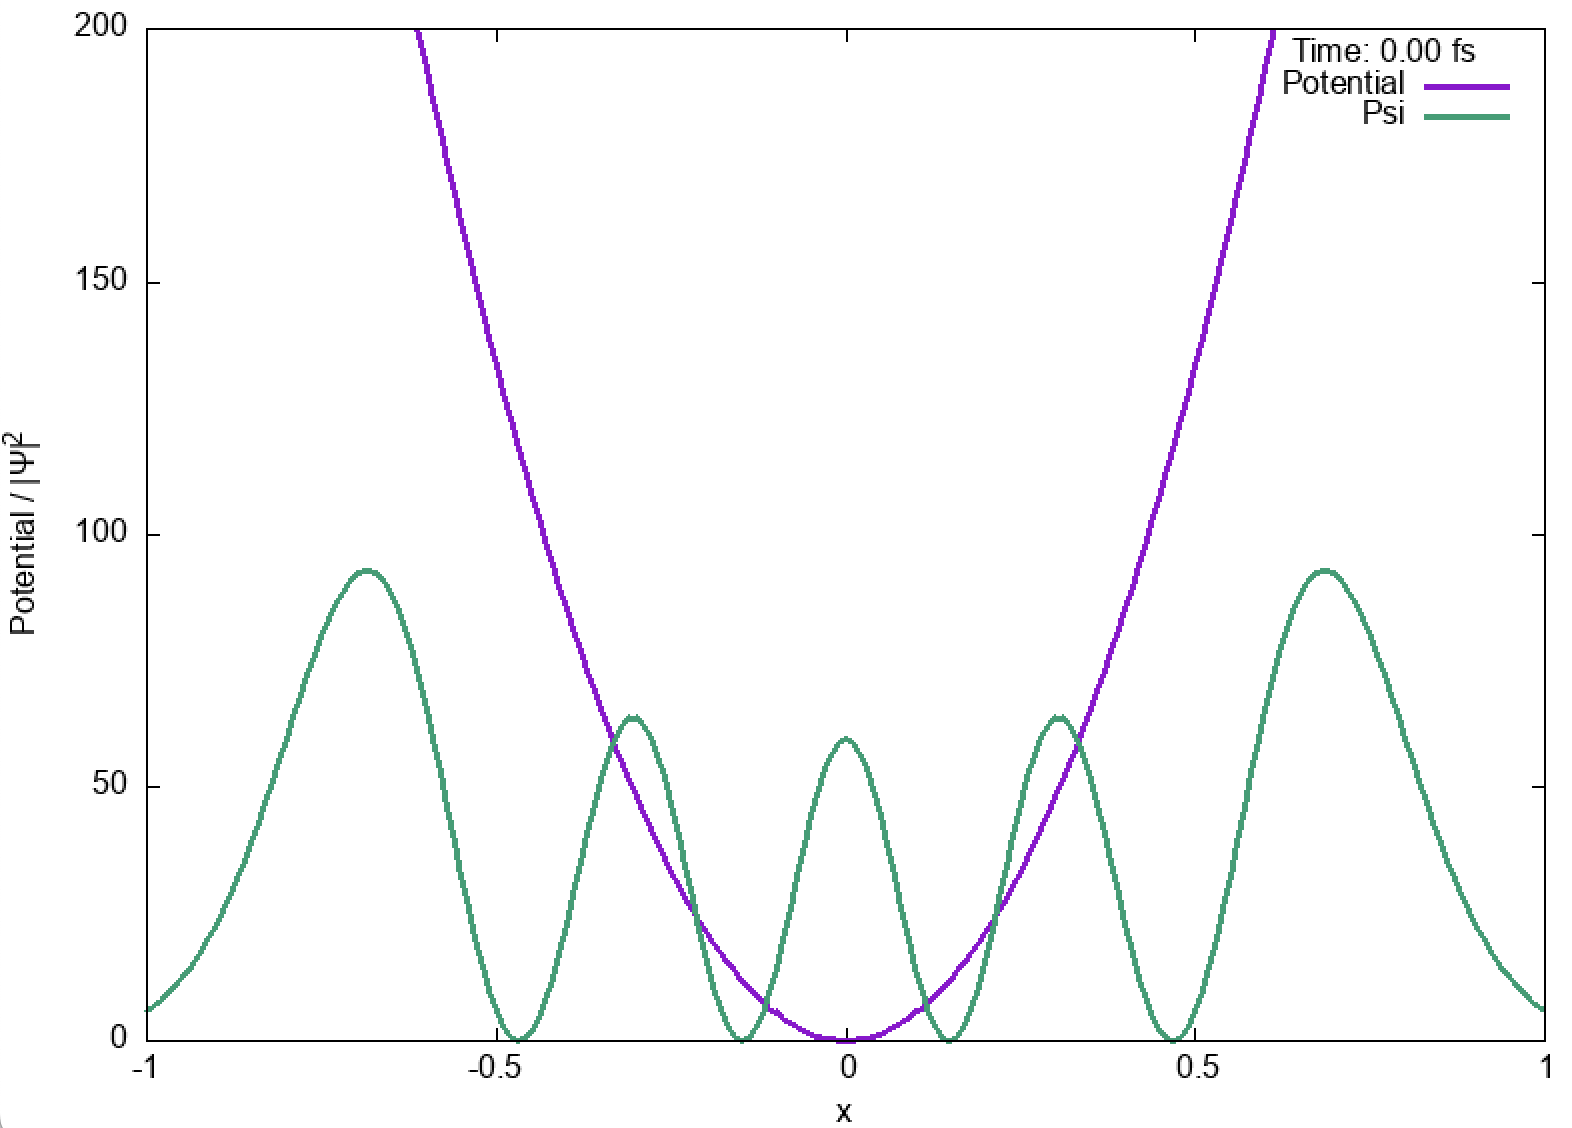
\includegraphics[width=0.33\textwidth]{H4.png}}
    \caption{Stationary $\abs{\Psi_n}^2$ made of a single Eigenfucntion $\Phi_n$}
    \label{fig:images}
\end{figure}

\section{Mixed Eigenfunctions}
When the wavefunction is in a superposition of eigenstates, the probability density will no longer be static as the frequency of each eigenstate is different:
\[
\Psi_{n}(x,t) = \sum_{n} c_n \cdot e^{-iE_nt} \cdot \Phi_{n}(x) = \sum_{n} c_n \cdot e^{-it\omega(n+\frac{1}{2})} \cdot \Phi_{n}(x)
\]

\[
\begin{aligned}
|\Psi_{n}(x,t)|^2 &= \left[\sum_{n} c_n e^{-iE_nt} \Phi_n(x)\right] \left[\sum_{n} c_n e^{iE_nt} \Phi_n(x)\right] \\
&= \sum_n |c_n|^2 |\Phi_n(x)|^2 + \sum_n \sum_{m>n} c_n c_m \Phi_n(x) \Phi_m(x) \cdot \left(e^{i(E_m-E_n)t}+e^{-i(E_m-E_n)t}\right) \\
&= \sum_n |c_n|^2 |\Phi_n(x)|^2 + 2\sum_n \sum_{m>n} c_n c_m \Phi_n(x) \Phi_m(x) \cdot \text{Re}\left(e^{-i(E_m-E_n)t}\right) \\
&= \sum_n |c_n|^2 |\Phi_n(x)|^2 + 2 \sum_n \sum_{m>n} c_n c_m \Phi_n(x) \Phi_m(x) \cdot \cos(t\omega(m-n))
\end{aligned}
\]
The resulting probability density is a function of time where each cross term oscilates with a frequency of $\omega \cdot (m-n)$. The overall period will be determined by the greatest common divisor (GCD) of the $(m-n)$ set, being $T=\frac{2\pi}{GCD_{\{m-n\}}\cdot\omega}$. \\
In this case, the fundamental angular frequency is 0.2825 fs$^{-1}$, giving a period of $T=22.23$ fs.\\
\par
The overall motion of the wavefunction will come from the constructive/destructive interference of its parent eigenfunctions. For instance, all even $\Phi_n$ have an antinode at the center, so we can expect a great variation in the probability density there. Bellow the cases for $\Psi = \ket{11111}$, $\Psi = \ket{10101}$ and $\Psi = \ket{01010}$ are explored.


\subsection{Case $\Psi = \ket{11111}$}

The wavefunction is initialized as a superposition of the first 5 eigenfunctions with equal weight. The probability density is plotted at different times in Figure \ref{fig:H11111}. The probability density oscilates with a period of $T=2\pi/\omega=22.23$ fs, as $GCD_{\{m-n\}}=1$. The overall motion would be that of a "travelling wave", without simmetry.
\begin{figure}[h!]
    \centering
    \subfloat[$t=0.0$ fs $(0 T)$]{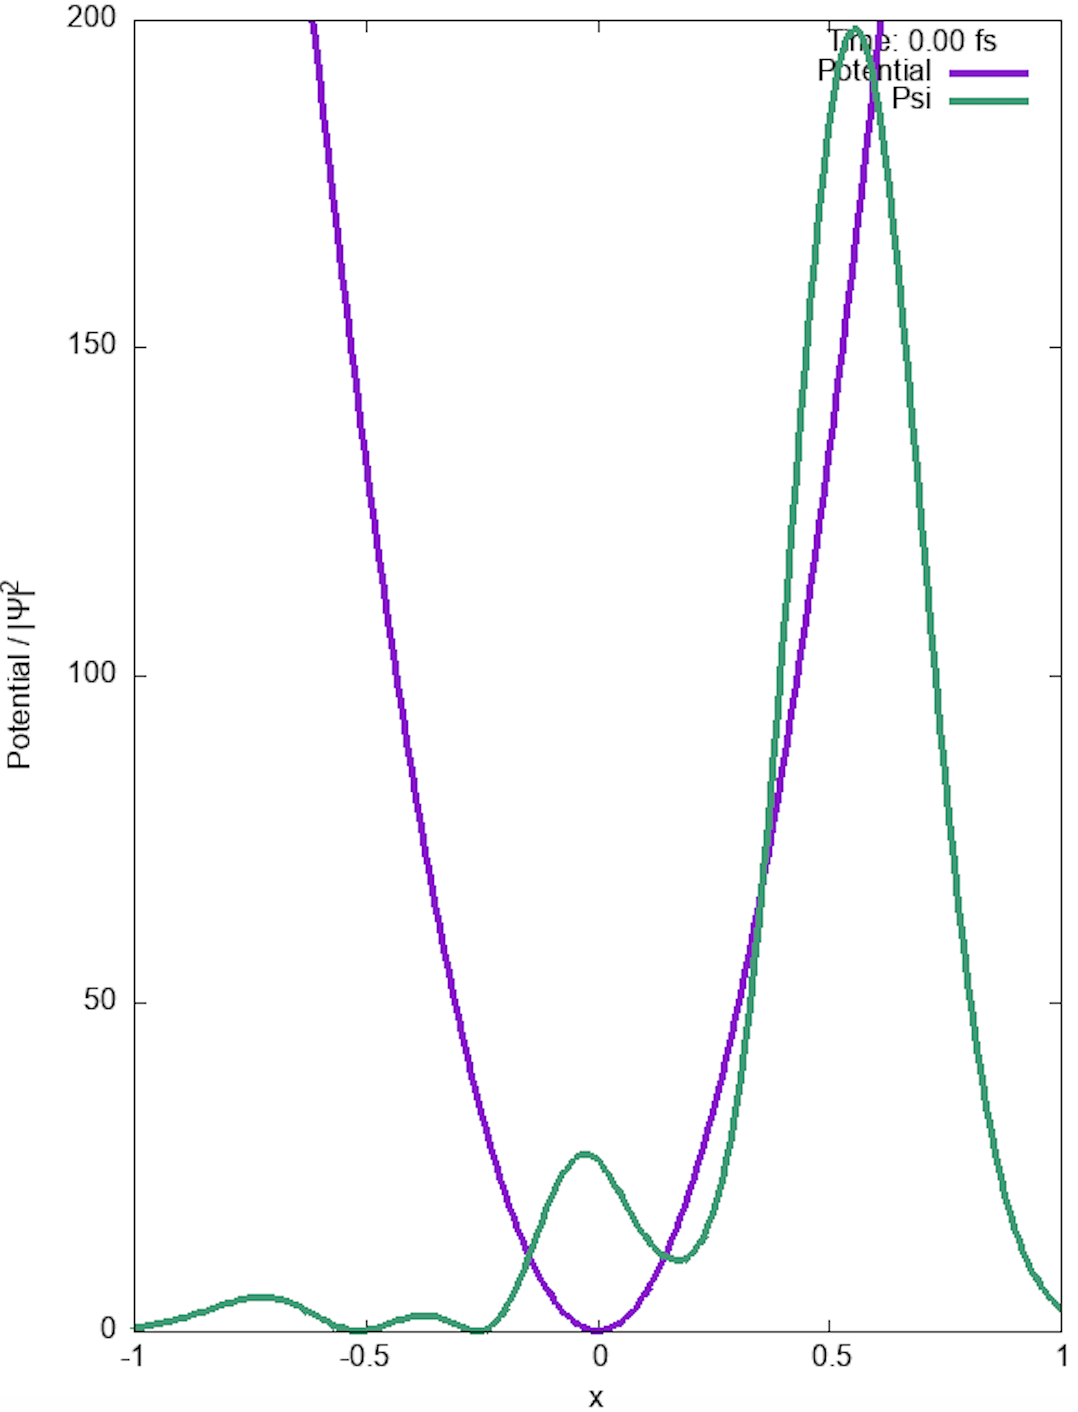
\includegraphics[width=0.25\textwidth]{H1_1.png}}
    \subfloat[$t=3.0$ fs $(0.13 T)$]{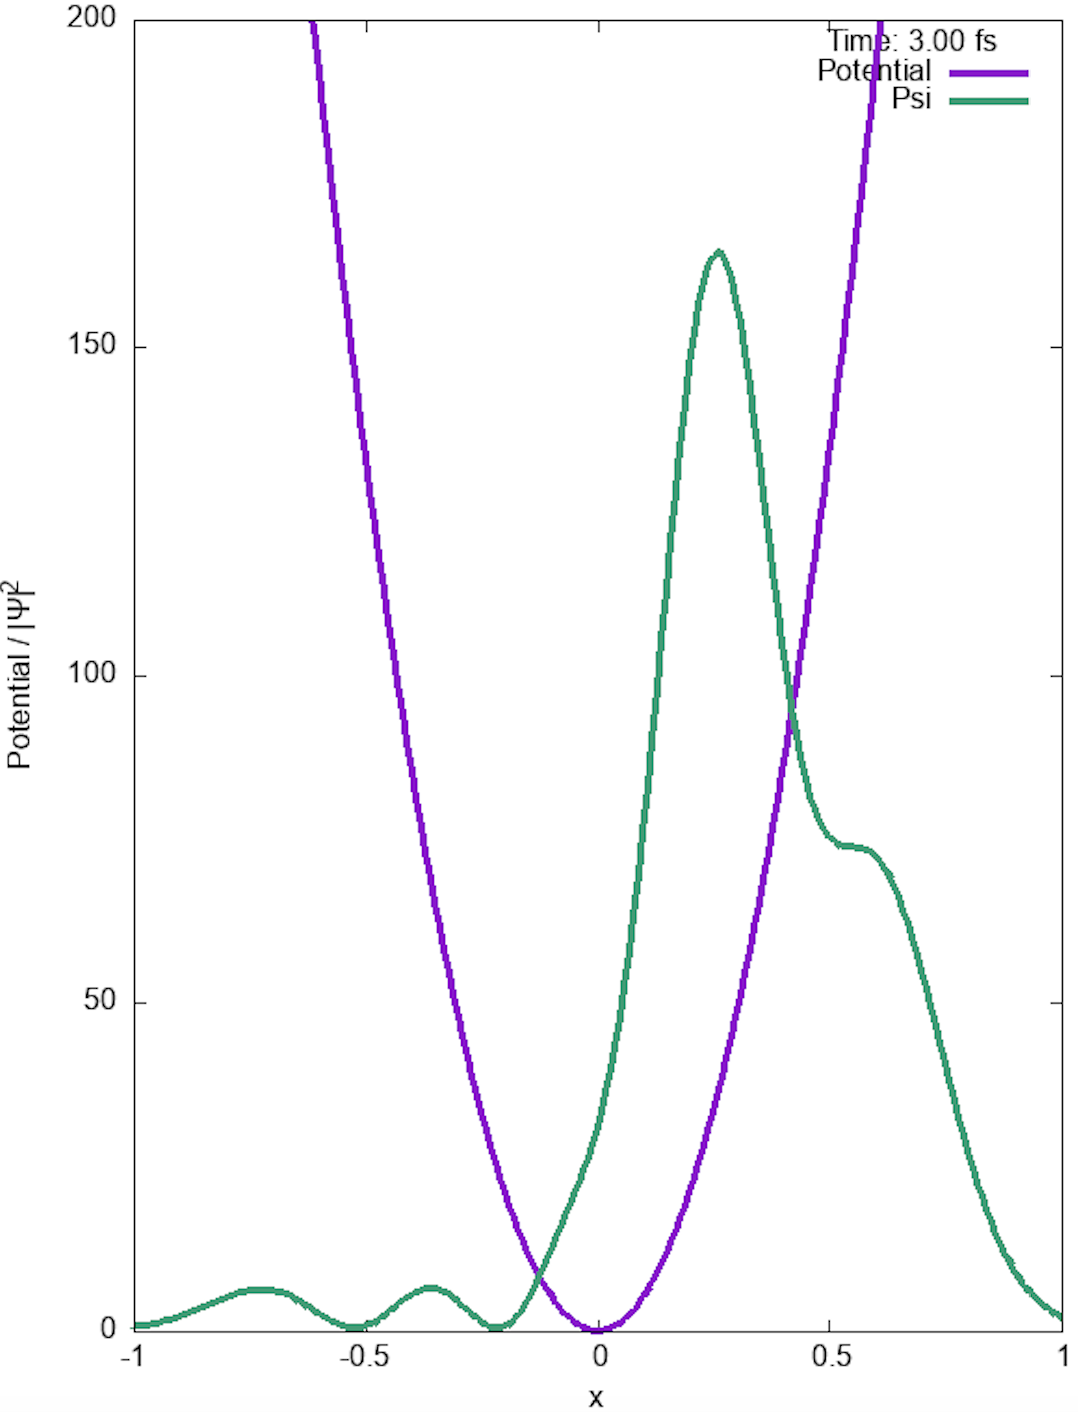
\includegraphics[width=0.25\textwidth]{H1_2.png}}
    \subfloat[$t=5.6$ fs $(0.25 T)$]{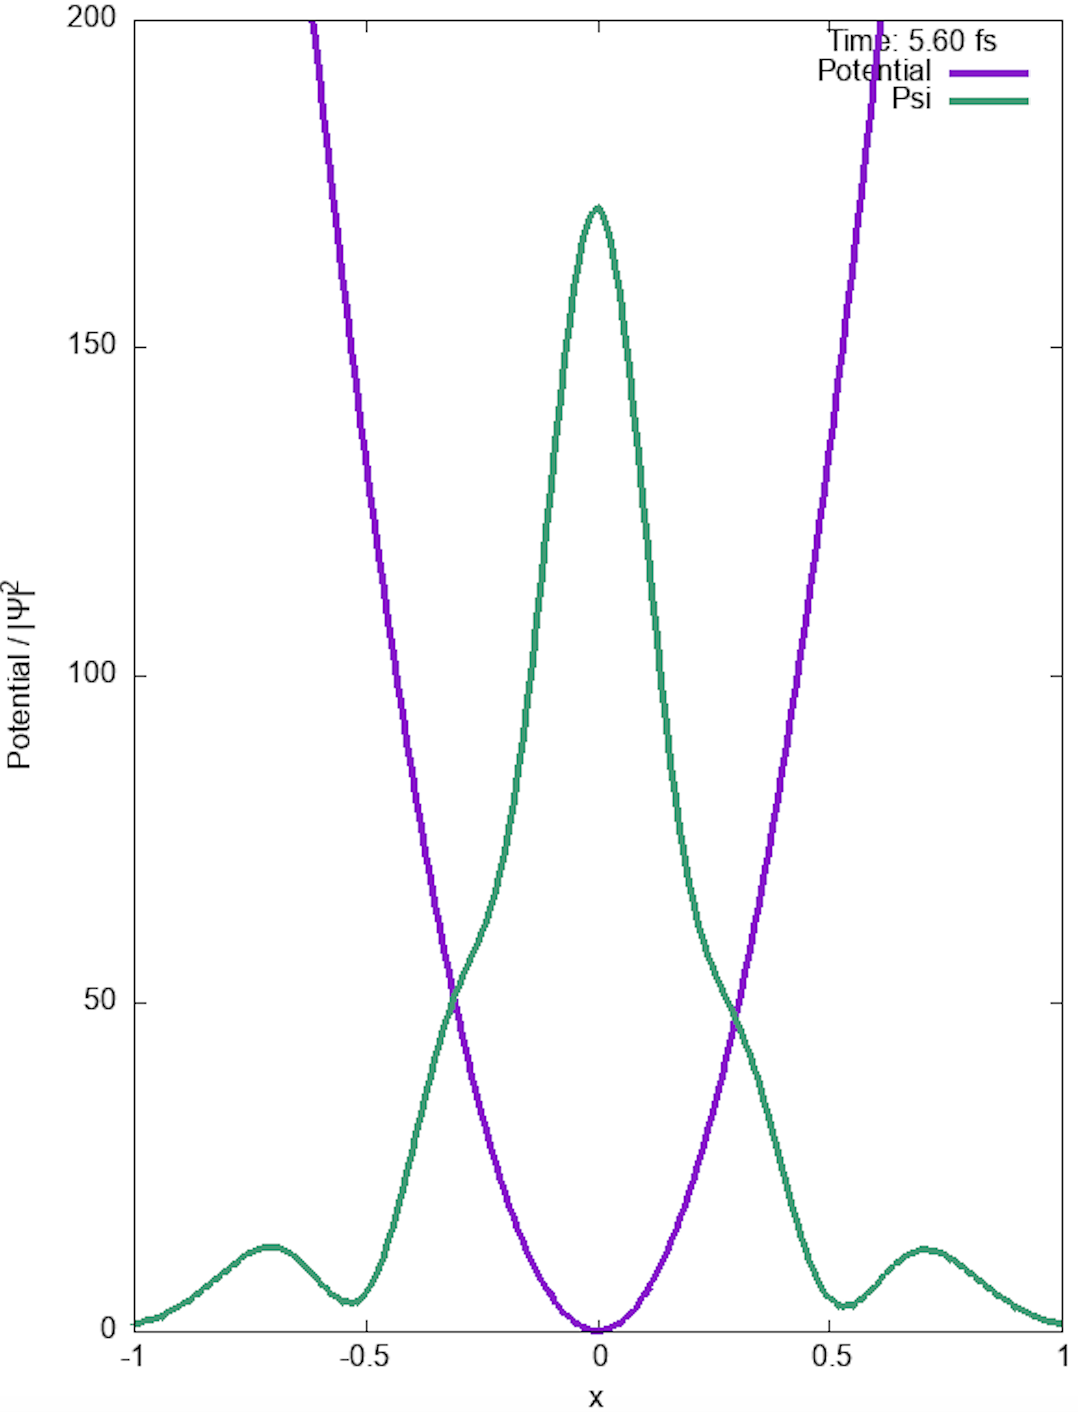
\includegraphics[width=0.25\textwidth]{H1_3.png}}
    \subfloat[$t=11.2$ fs $(0.5 T)$]{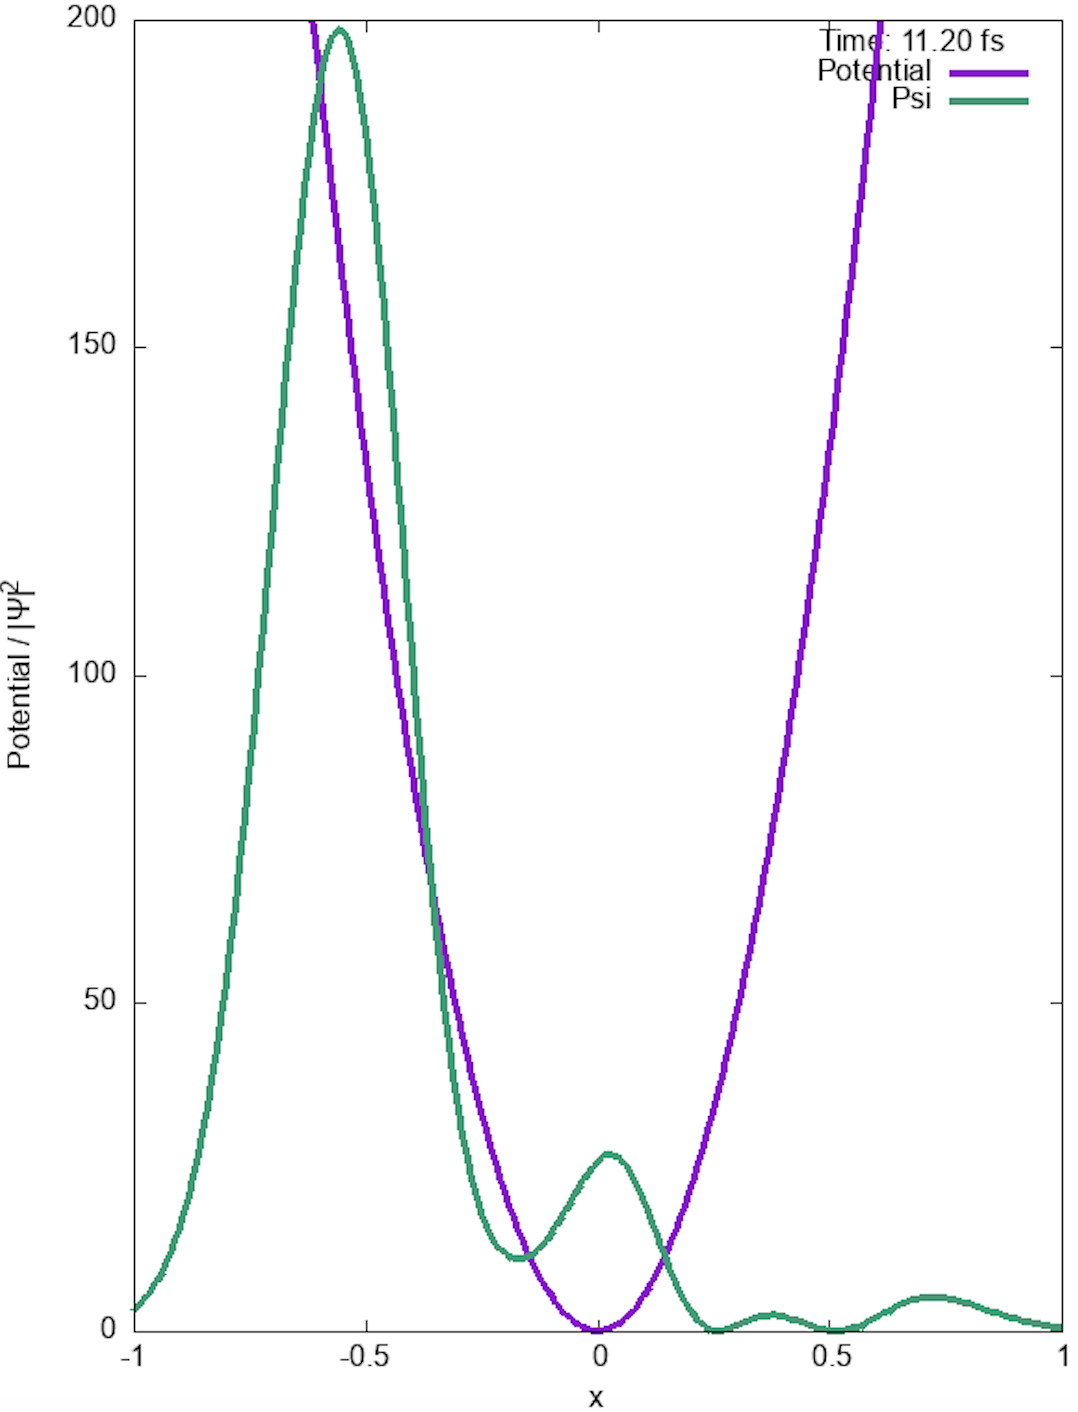
\includegraphics[width=0.25\textwidth]{H1_4.png}}
    \caption{Time evolution for $\Psi = \ket{11111}$. Its period is $T=2\pi/\omega=22.23$ fs}
    \label{fig:H11111}
\end{figure}

\subsection{Case $\Psi = \ket{10101}$}

The wavefunction is initialized as a superposition of the first 3 even eigenfunctions with equal weight. The probability density is plotted at different times in Figure \ref{fig:H10101}. The probability density is oscilates with a period of $T=\pi/\omega=11.12$ ( $GCD_{\{m-n\}}=2$). Its movement is that of a standing wave, symmetric around its center but without nodes. Because all the components are even functions, all contribute with an antinode in the center, and we can observe the greatest interference there.
\begin{figure}[h!]
    \centering
    \subfloat[$t=0.0$ fs $(0 T)$]{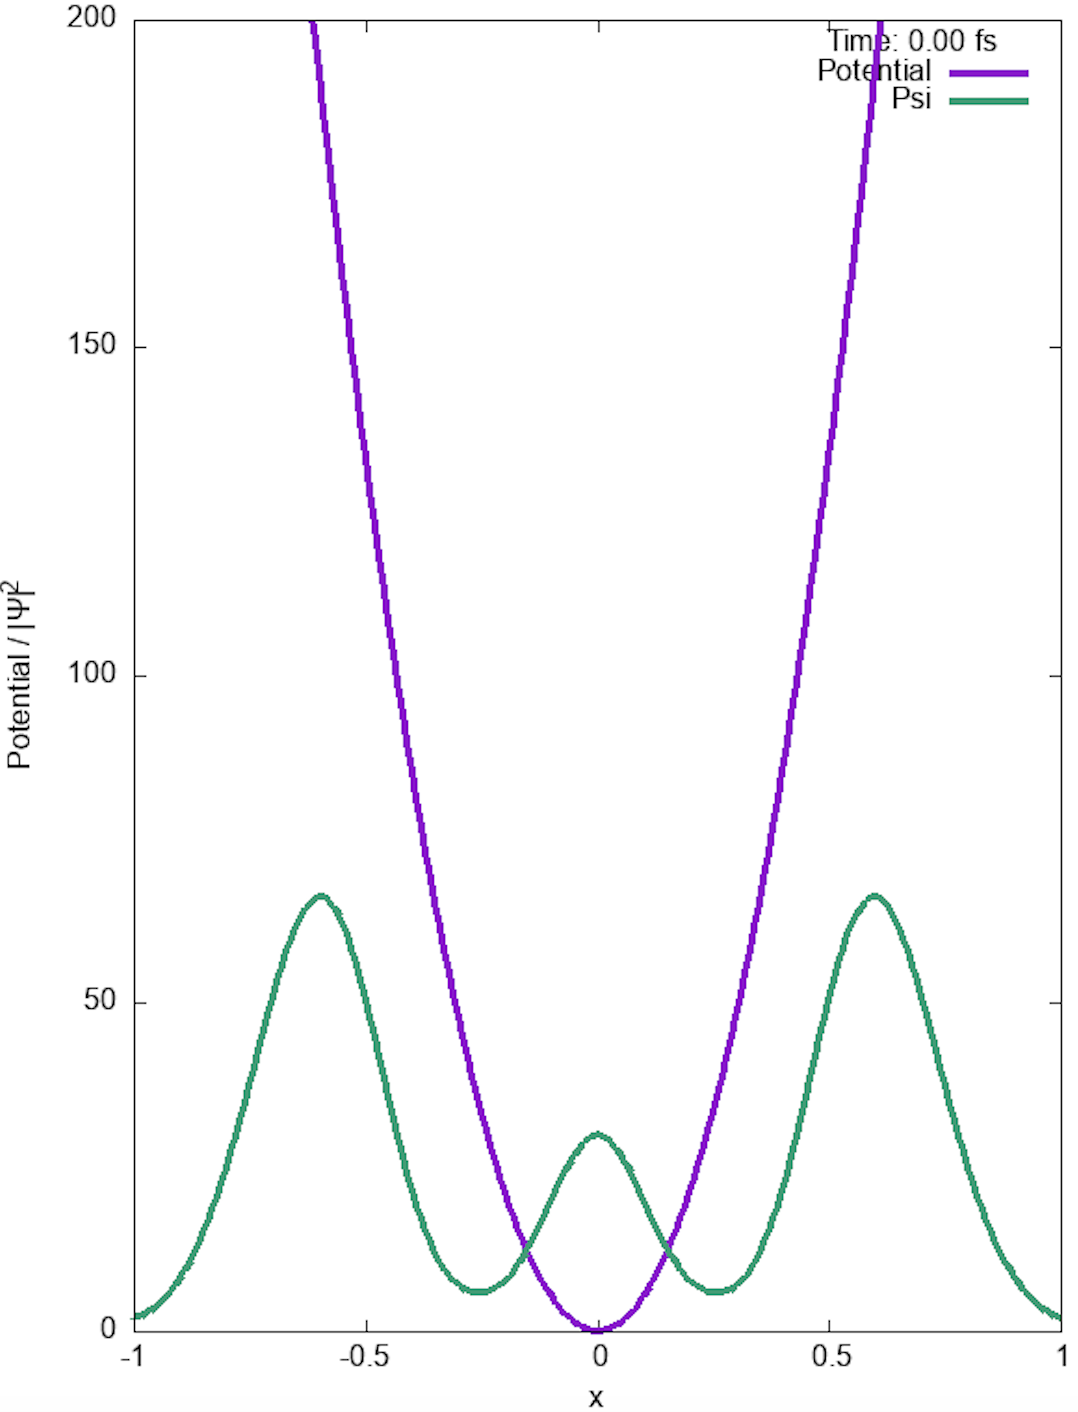
\includegraphics[width=0.25\textwidth]{H2_1.png}}
    \subfloat[$t=1.8$ fs $(0.16 T)$]{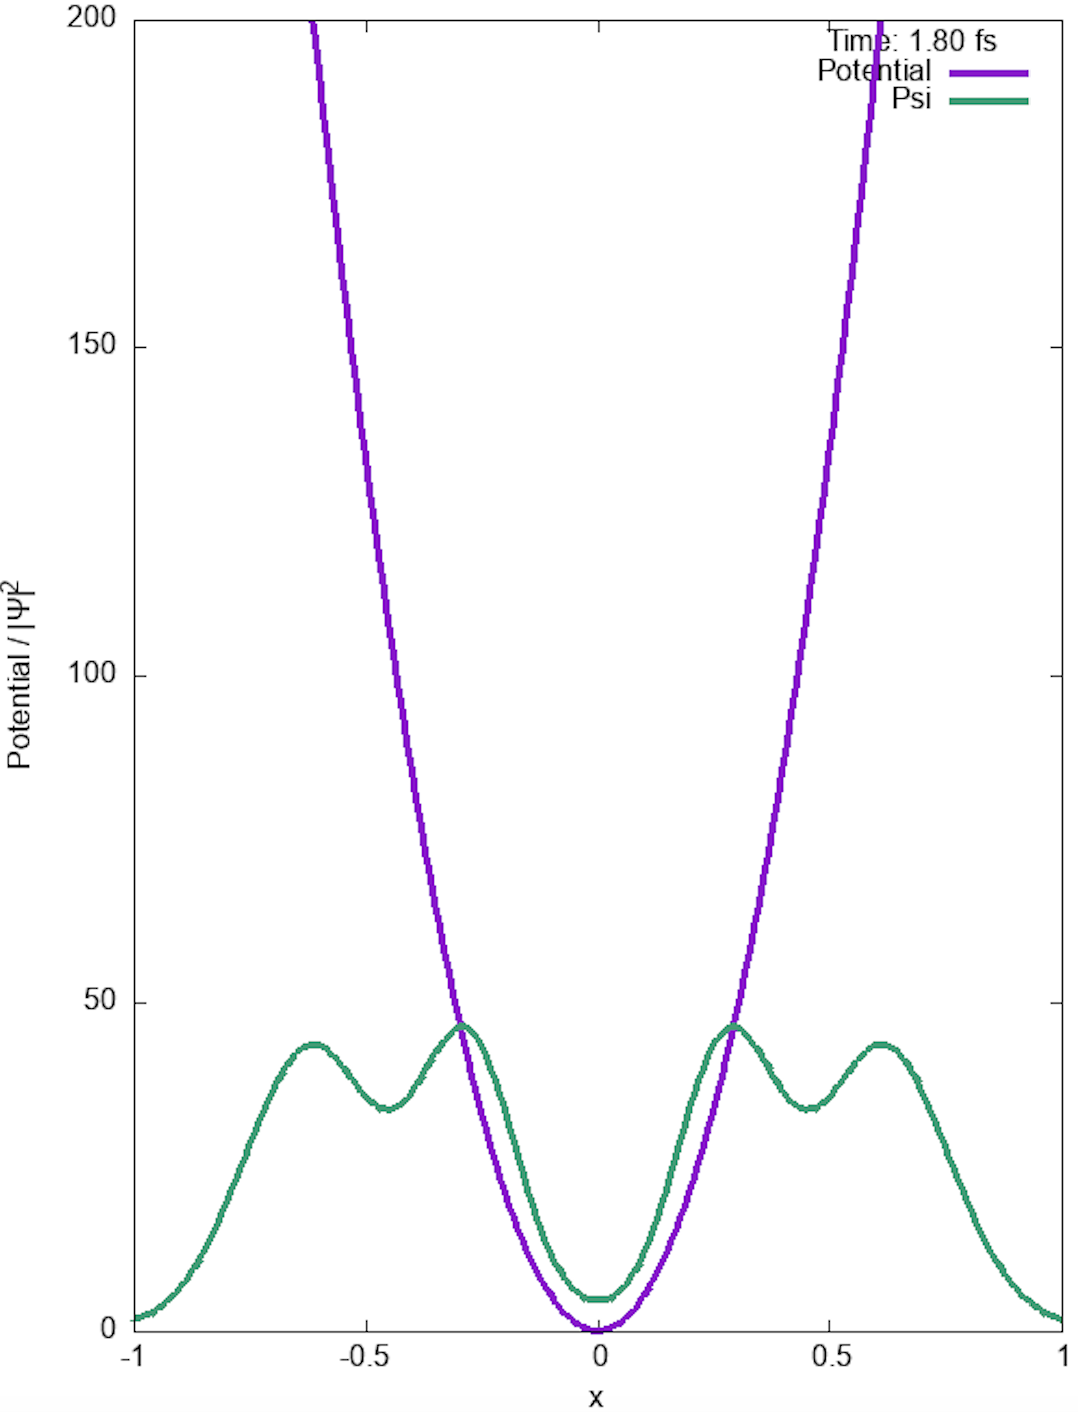
\includegraphics[width=0.25\textwidth]{H2_2.png}}
    \subfloat[$t=2.8$ fs $(0.25 T)$]{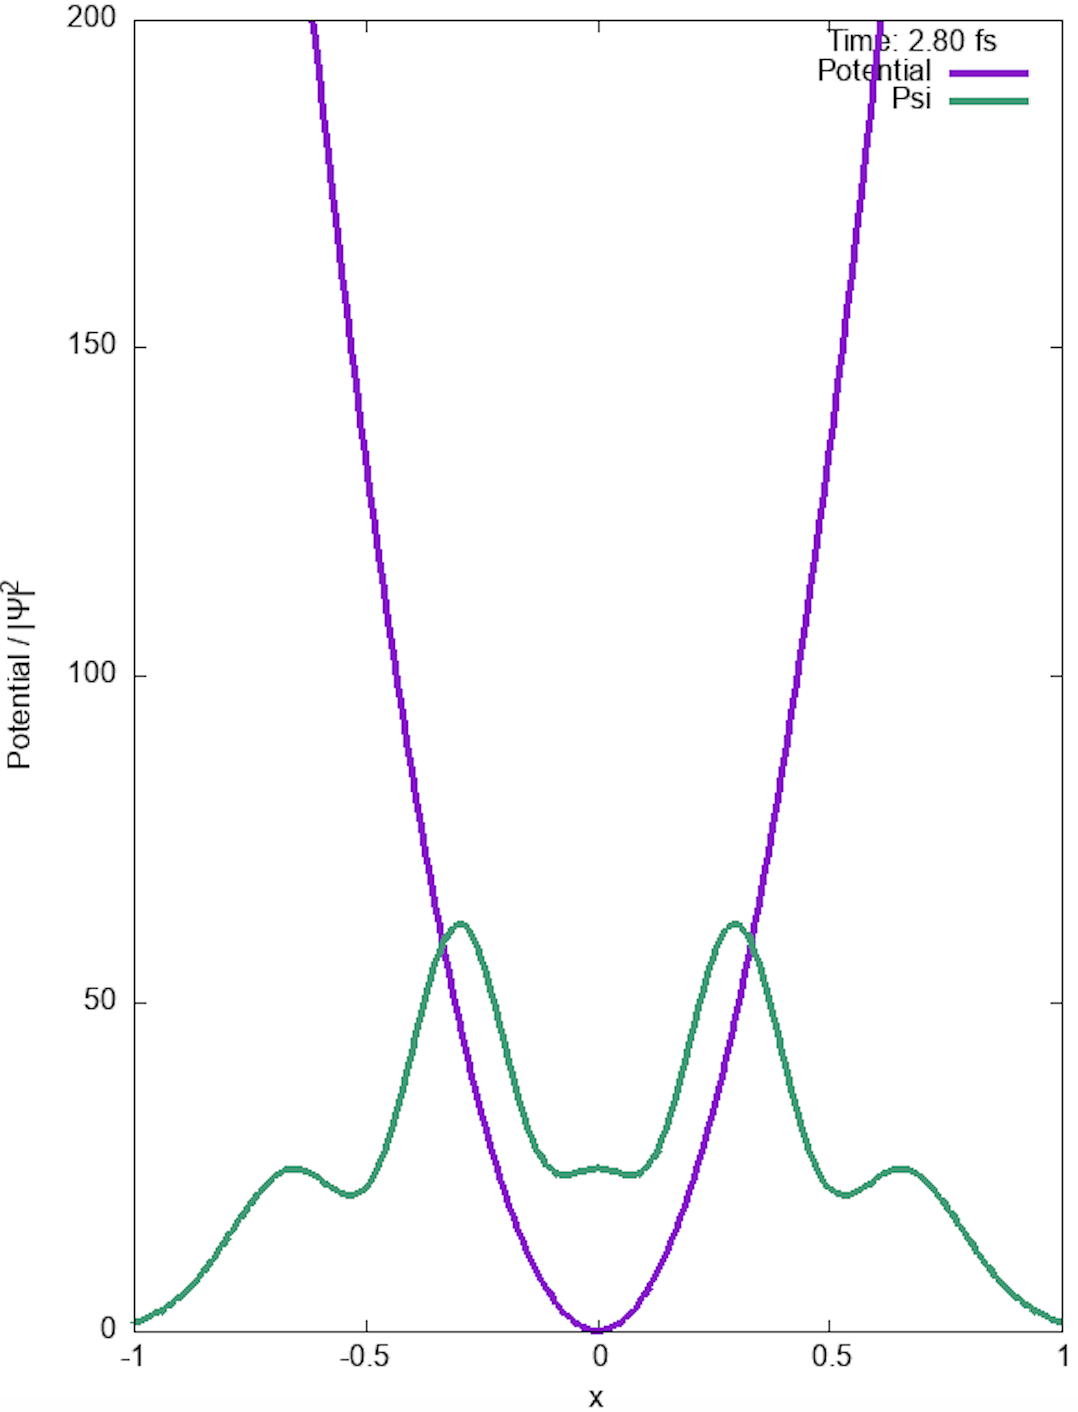
\includegraphics[width=0.25\textwidth]{H2_3.png}}
    \subfloat[$t=5.60$ fs $(0.5 T)$]{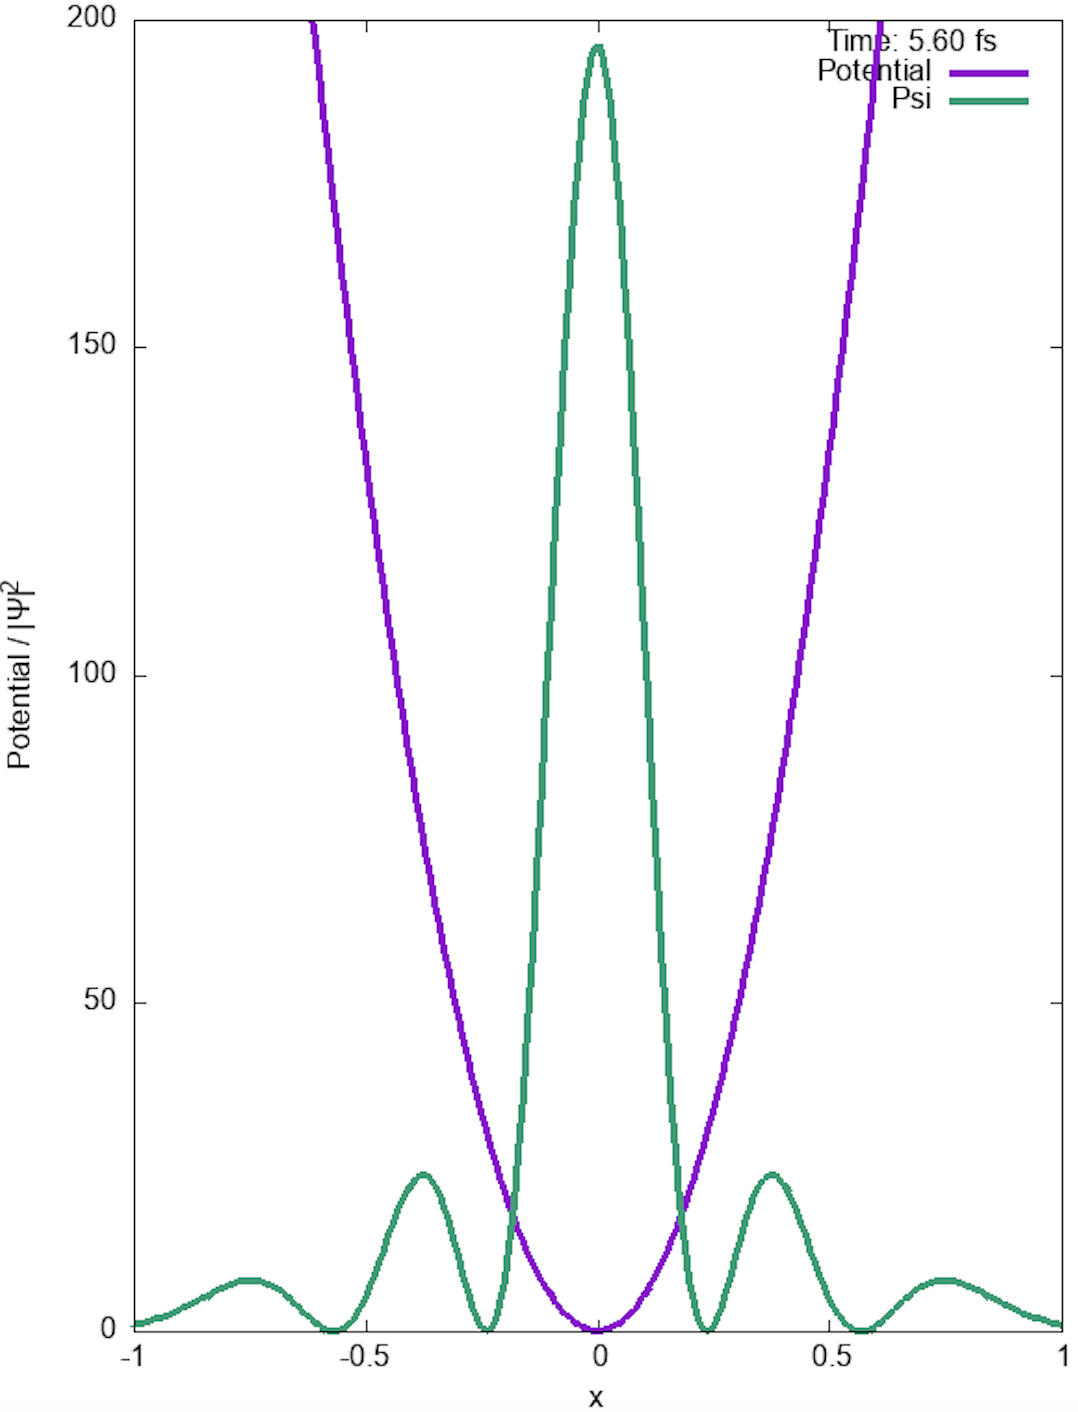
\includegraphics[width=0.25\textwidth]{H2_4.png}}
    \caption{Time evolution for $\Psi = \ket{10101}$. Its period is $T=\pi/\omega=11.12$ fs}
    \label{fig:H10101}
\end{figure}

\subsection{Case $\Psi = \ket{01010}$}

The wavefunction is initialized as a superposition of the first 2 odd eigenfunctions with equal weight. The probability density is plotted at different times in Figure \ref{fig:H01010}. The probability density oscilates with a period of $T=\pi/\omega=11.12$ fs ( $GCD_{\{m-n\}}=2$).  Its movement is that of a standing wave, symmetric around its center with a node in the middle. In contrast to the previous case, we see this node as the parent functions also contain that node.
\begin{figure}[h!]
    \centering
    \subfloat[$t=0.0$ fs $(0 T)$]{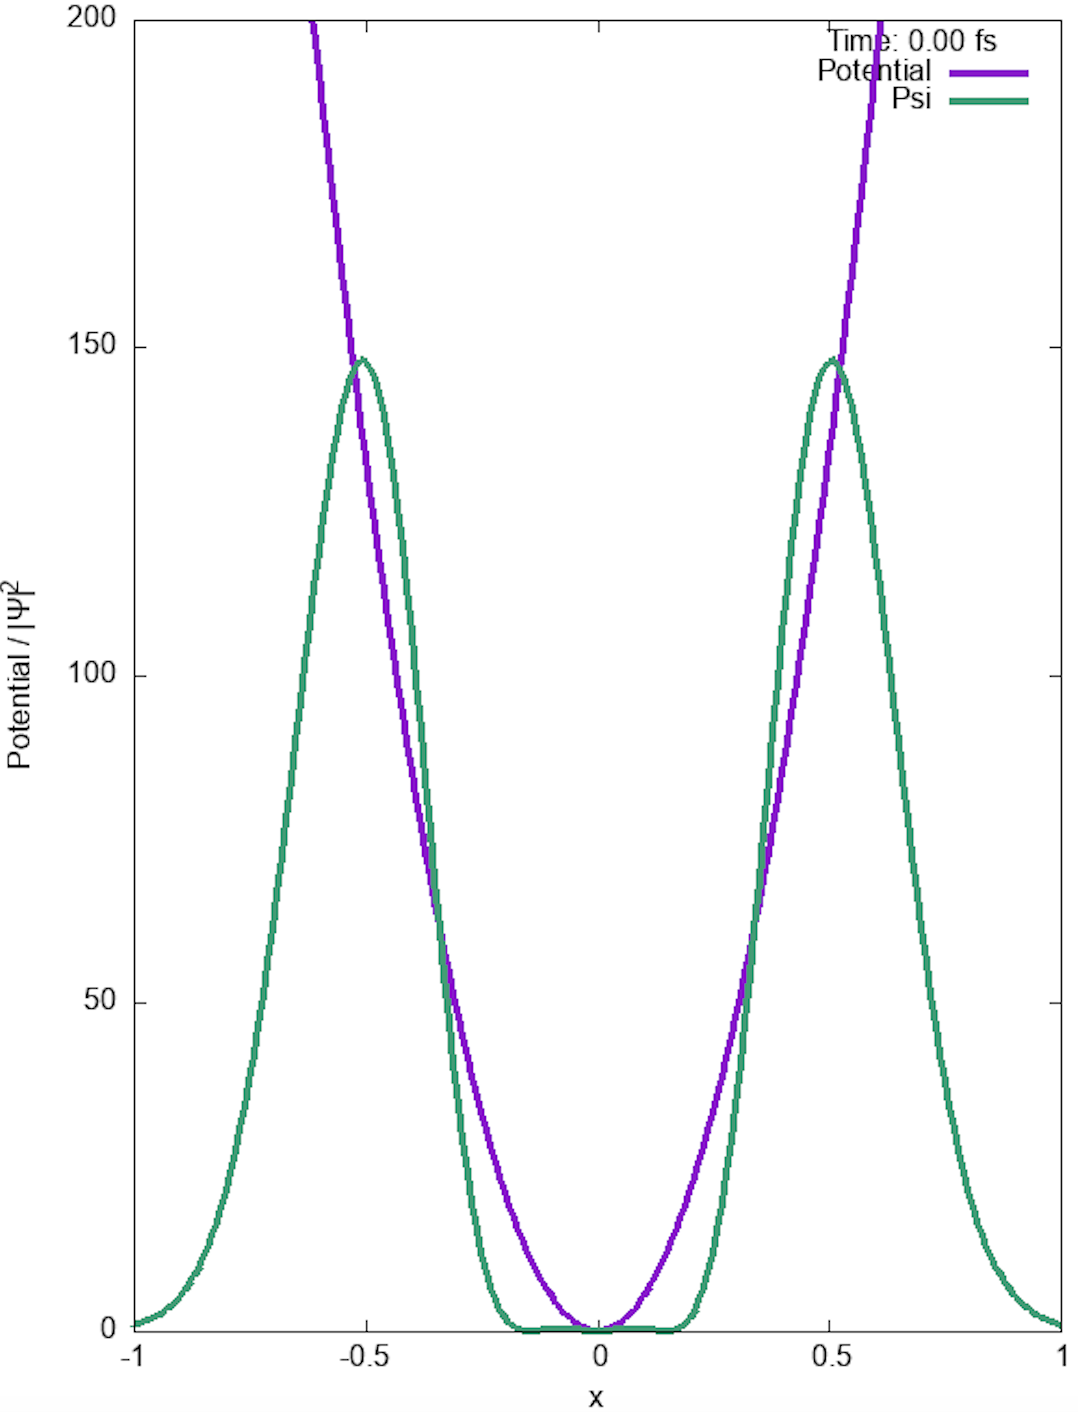
\includegraphics[width=0.25\textwidth]{H3_1.png}}
    \subfloat[$t=1.8$ fs $(0.16 T)$]{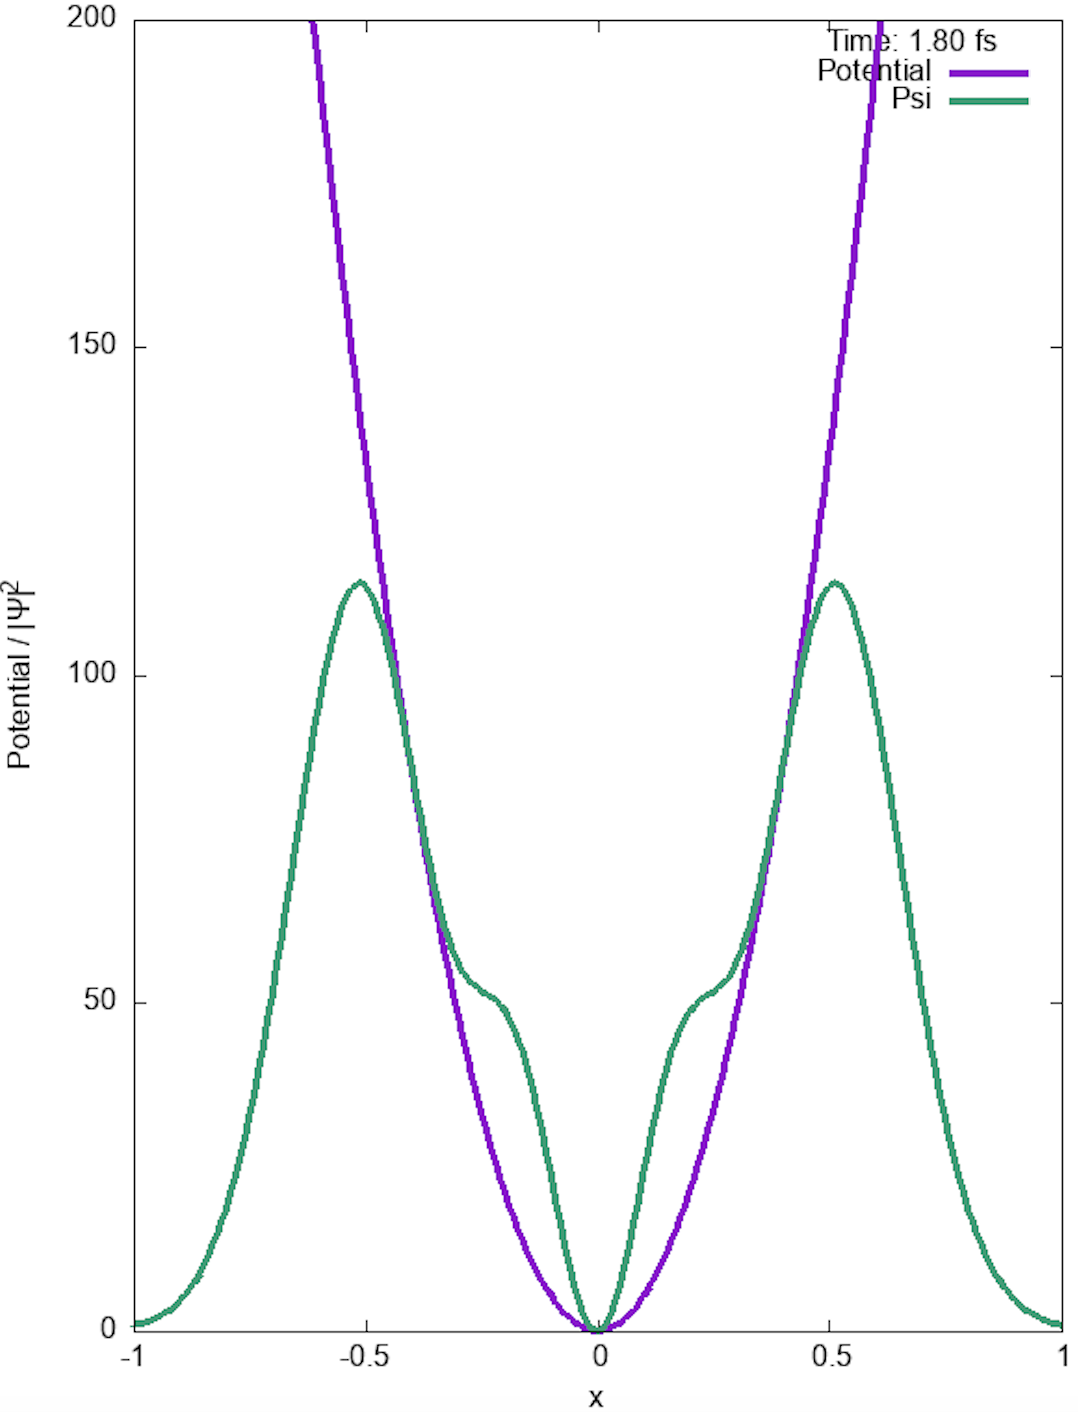
\includegraphics[width=0.25\textwidth]{H3_2.png}}
    \subfloat[$t=3.0$ fs $(0.25 T)$]{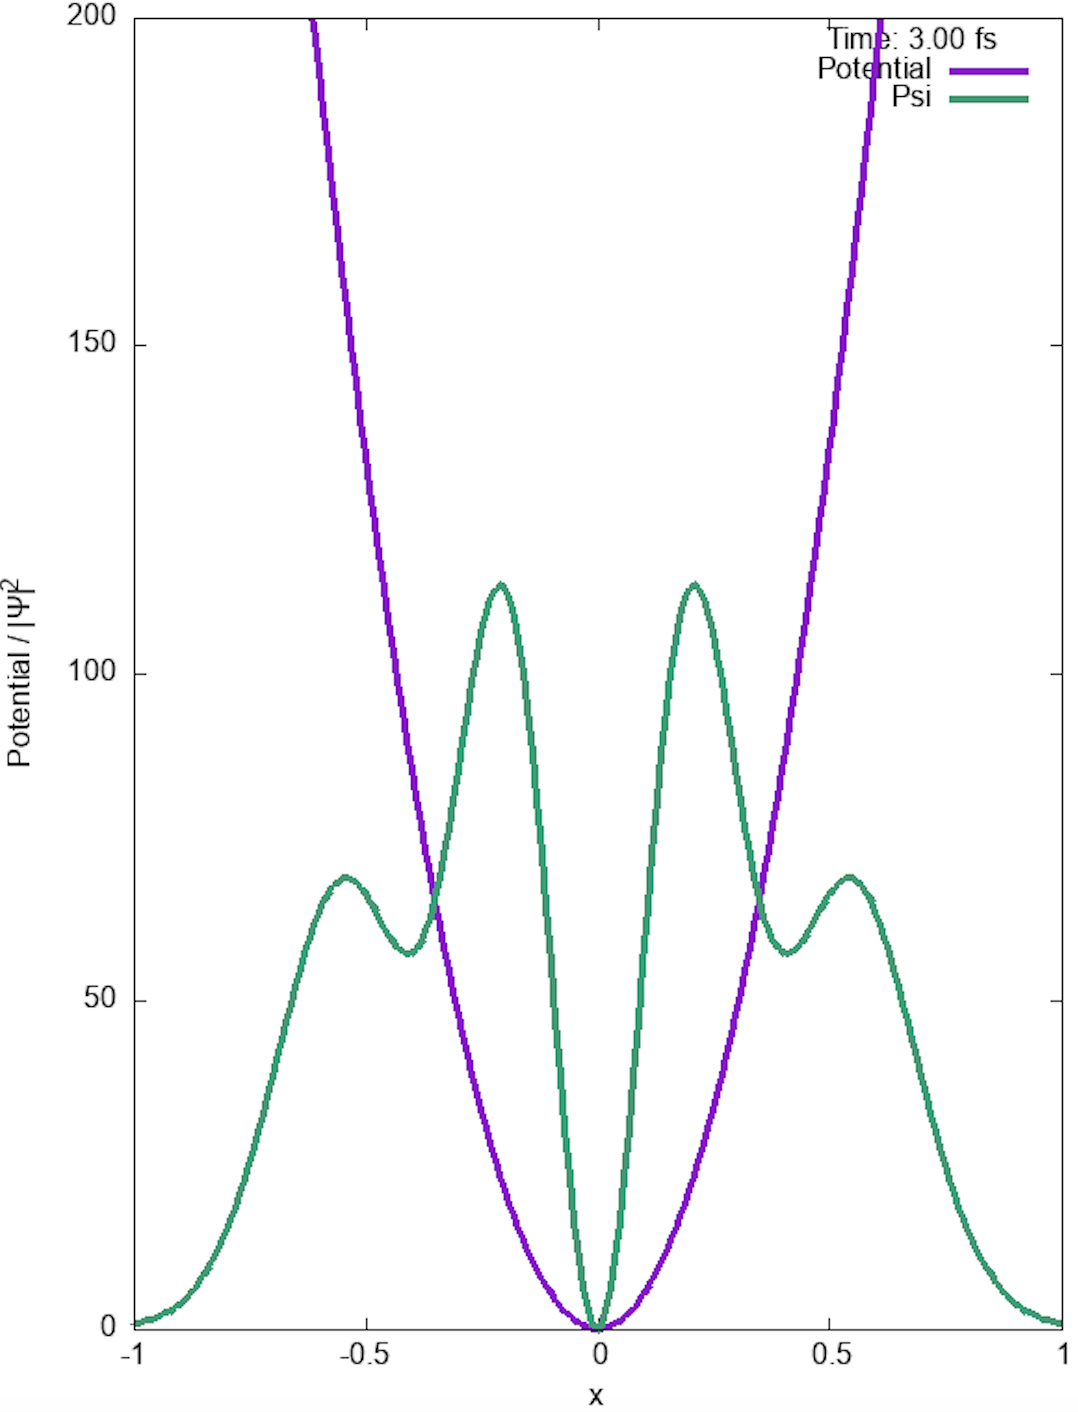
\includegraphics[width=0.25\textwidth]{H3_3.png}}
    \subfloat[$t=5.60$ fs $(0.5 T)$]{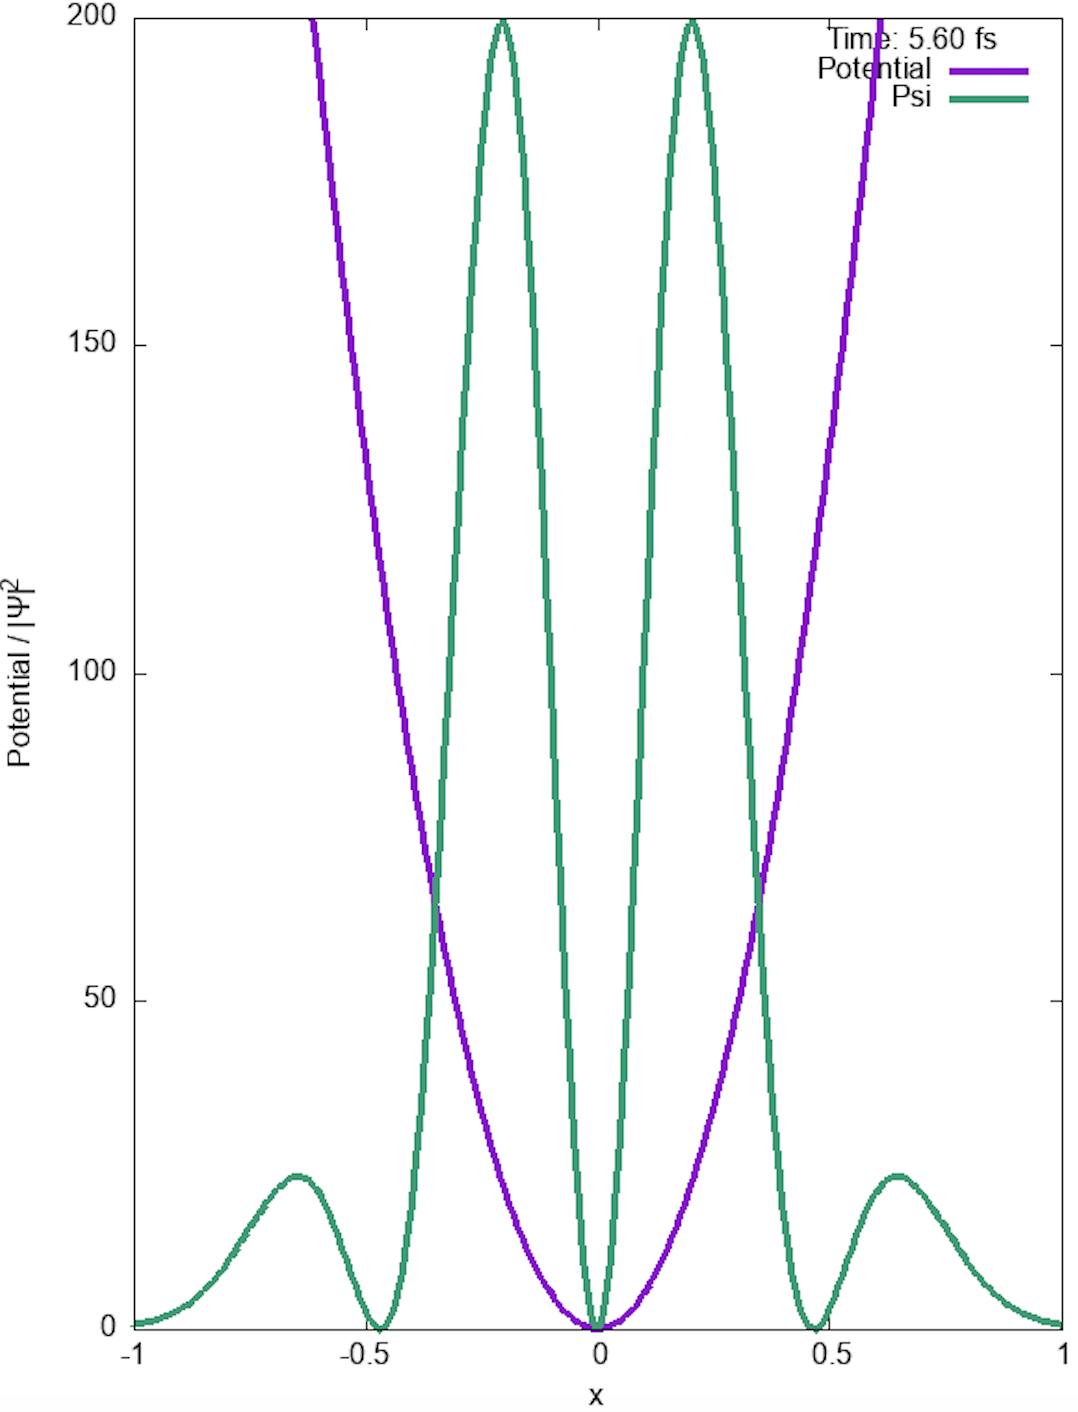
\includegraphics[width=0.25\textwidth]{H3_4.png}}
    \caption{Time evolution for $\Psi = \ket{01010}$. Its period is $T=\pi/\omega=11.12$ fs}
    \label{fig:H01010}
\end{figure}

\end{document}

We can easily check this in the code by plotting the real part of the projection of $\Psi$ over $\Phi_n$ over time:\\
\[
\mathbb{Re}(c'_n(t)) = \mathbb{Re} \left( \bra{\Phi_n} \ket{\Psi} \right) = \mathbb{Re} \left( c_n e^{-i\omega(n+\frac{1}{2})t}\bra{\Phi_n}\ket{\Phi_n} \right) = c_n \cos\left(\omega(n+\frac{1}{2})t\right)
\]
